\chapter{Introduction}
\setcounter{page}{1}

\section{Background and Motivation}

In the 21st century, climate change is the biggest challenge faced by humanity.
It poses a substantial danger to the survival of the inhabitants of our planet.
Human activities such as deforestation, extraction and burning of fossil fuels have led to a rise in global temperatures.
The consequences of such activities are an increase in sea levels, extreme weather events, and loss of biodiversity.
There is an urgent and undeniable need to reduce greenhouse gas emissions and transition to a sustainable and low-carbon future.

Maritime shipping is essential to the global economy.
It accounts for transporting 90\% of the world's goods by volume.
It is also a major source of greenhouse gas emissions,
with the International Maritime Organization (IMO) estimating that maritime shipping accounts for 3\% of global carbon dioxide emissions.
While 3\% may seem small, it is important to note that this is a rapidly growing sector.
Without action, maritime shipping contribution to carbon emissions can increase by up to 10-13\% in the next few decades.
Due to this fact, there is a growing global effort to reduce emissions from this sector. \autocite{king_anthony_2022}.

The European Green Deal is a significant initiative by the European Union to make Europe the world's first climate-neutral continent by 2050 .
It aims to transform various sectors, including shipping, to reduce environmental impacts.
Through meticulous analysis of total carbon emissions within the maritime sector using advanced data techniques,
this research can significantly contributes to the goals of the European Green Deal. It can aid in formulating policies, monitoring progress, and promoting sustainable practices,
aligning with the Green Deal's emphasis on innovation, global cooperation, and eco-conscious industrial transformation \autocite{siddi2020european}.
This study's alignment with the European Green Deal underscores its relevance and importance within the broader context of sustainability-focused endeavors.

In accordance with Sustainable Development Goal 13, in 2018, the initial strategy was adopted by IMO's Environmental Protection Committee (MEPC),
during its 72nd session at IMO Headquarters in London, United Kingdom. According to this strategy,
the IMO will work towards reducing the total annual greenhouse gas emissions from international shipping by at least 50\% by 2050 compared to 2008 \autocite{imo-2018}.
In the 76th session of MEPC in 2021, serval mandatory measures were adopted to reduce greenhouse gas emissions from international shipping,
which will help in achieving the goal of reducing emissions by 50\% by 2050 \autocite{imo-2021}.
One of the important measures is the Carbon Intensity Indicator (CII).

Maritime shipping is a complex and highly volatile system, generating very large data sets.
Big data analytics can be used to understand the complex system and make informed decisions.
It can facilitate operations such as monitoring of emissions and predictive analysis of vessel performance.
This can help in reducing emissions and improving the efficiency of the maritime sector \autocite{ZAMAN2017537}.

\begin{figure}[ht]
    \centering
    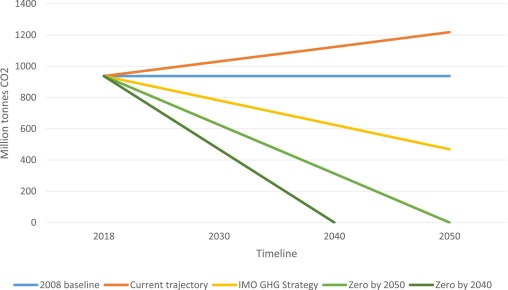
\includegraphics[width=0.7\textwidth]{images/emission_trajactory.jpg}
    \caption{Emission trajectories for different levels of ambition for emission reduction targets}
    \label{emissionTrajectory}
\end{figure}


\section{Big Data Analysis}

Big data analytics is where advanced analytic techniques operate on big data sets. Hence, big data
analytics is really about two things — \textit{big data} and \textit{analytics}.



\subsection{Big Data}

As the name suggests, big data is a large amount of data. There are other important attributes of big data. These are:  data variety and data velocity.

Thus we can define big data using 3 V's: \textit{volume}, \textit{variety}, and \textit{velocity} as showin in figure \ref*{bigData}.

\begin{figure}[h]
    \centering
    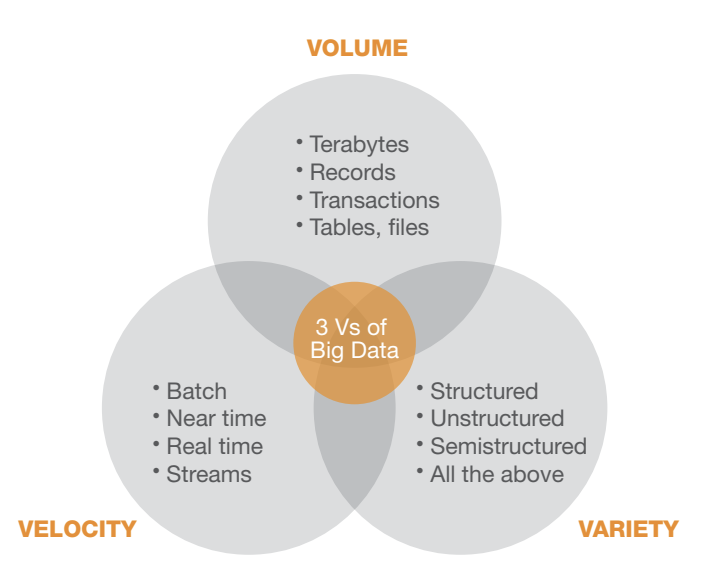
\includegraphics[width=0.5\textwidth]{images/big_data.png}
    \caption{Big Data: 3 V's \autocite{3vbigdata}}
    \label{bigData}
\end{figure}

Beyond these three V's, Big Data is also about how complicated the computing
problem is. Given the number of variables and number of data points for analysing the maritime shipping data. It is a very complicated problem.
Thus, in addition to the three V's identified by IBM, it would also be necessary to take complexity into account as shown in figure \ref*{bigDataComplex} \autocite{pence2014big}.

\begin{figure}[h]
    \centering
    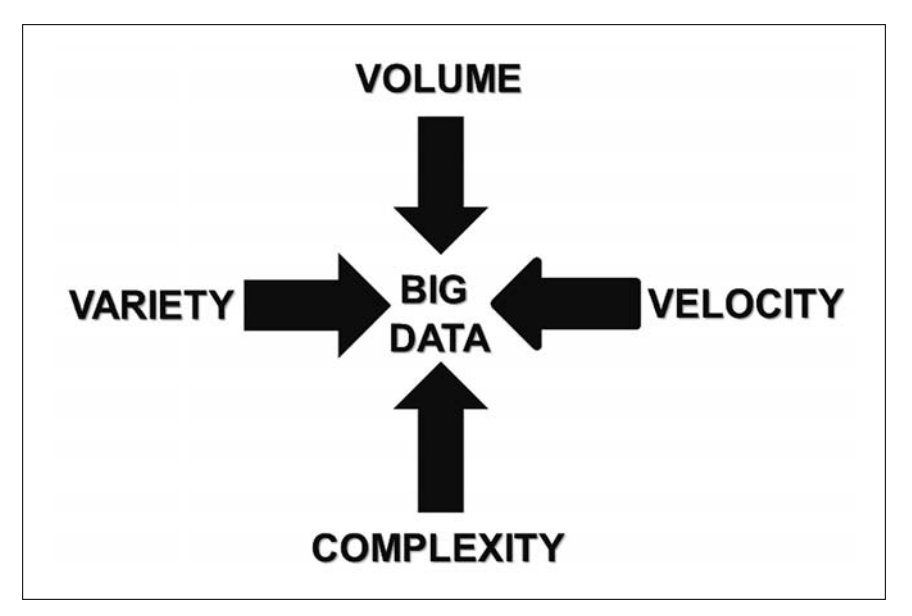
\includegraphics[width=0.5\textwidth]{images/big_data_complex.png}
    \caption{Big Data: Beyong 3 V's - volume, velocity,
        variety, and complexity}
    \label{bigDataComplex}
\end{figure}


\subsection{What is Big Data Analytics?}

Big data analytics is the process of examining large and varied data sets to uncover hidden patterns, unknown correlations, market trends, customer preferences and other useful information that can help organizations make more-informed business decisions.

Thus, Data analytics revolves around deriving valuable knowledge and meaningful insights from extensive sets of data.
This process involves crafting hypotheses, often rooted in gathered experiences and uncovering correlations between variables, sometimes even through serendipitous discoveries.
Data analytics can be classified into four distinct types \autocite{rajaraman2016big}:

\subsubsection{1. Descriptive Analytics}

Descriptive analytics focuses on explaining past events and presenting them in a comprehensible manner.
The collected data is structured into visual aids like bar charts, graphs, pie charts, maps, and scatter diagrams, facilitating easy interpretation that offers insights into the data's implications.
This mode of data representation is often termed a dashboard, reminiscent of a car's dashboard that provides details such as speed, engine status, fuel levels, and distance traveled.
A classic instance of descriptive analytics involves displaying population census data, which categorizes a nation's population by gender, age brackets, education, income, population density, and similar criteria \autocite{rajaraman2016big}.

\subsubsection{2. Predictive Analytics}

Predictive analytics extends beyond existing data to forecast forthcoming events.
It anticipates what is likely to occur in the immediate future.
Techniques like time series analysis utilizing statistical methods, neural networks, and machine learning algorithms are employed for this extrapolation.
A significant application of predictive analytics is seen in marketing, where it understands customer preferences and needs.
For instance, when purchasing shoes online, an advertisement for socks may appear.
Another prevalent application is in orchestrating election campaigns.
This involves gathering diverse data, such as the demographics of voters in different areas and their perceived needs like infrastructure and local concerns \autocite{rajaraman2016big}.

\subsubsection{3. Prescriptive Analytics}

This process detects opportunities for enhancing existing solutions by analyzing collected data.
Essentially, it guides us on the actions to undertake in order to accomplish a particular objective.
An illustrative instance is observed in the aviation industry where airlines determine seat pricing through analysis of historical travel patterns, popular travel origins and destinations, significant events, holidays, and more.
This approach is employed to optimize profit generation \autocite{rajaraman2016big}.

\subsubsection{4. Exploratory or Discovery Analytics}

This process uncovers unforeseen connections among variables within extensive datasets.
The collection and analysis of data from diverse sources opens up new avenues for gaining insights and making serendipitous discoveries.
One of its major applications involves the identification of patterns in customers' behavior by companies through sources like feedback, tweets, blogs, Facebook data, emails, and sales trends.
By deciphering customer behavior, companies can potentially predict actions like renewing a magazine subscription, switching mobile phone service providers, or canceling a hotel reservation. Armed with this information, companies can devise appealing offers aimed at altering the anticipated course of action by the customer \autocite{rajaraman2016big}.
\section{Indicators}

Indicators play a crucial role in assessing and monitoring carbon emissions in the maritime shipping industry.
They provide valuable insights into the environmental performance of vessels,
facilitate comparisons between different ships or fleets, and help track progress towards emission reduction targets.
By measuring various aspects of emissions and energy efficiency,
these indicators enable stakeholders to identify opportunities for improvement and implement effective strategies to mitigate the environmental impact of shipping operations.

In this section, we will discuss several key indicators commonly used in the monitoring and evaluation of carbon emissions in maritime shipping.
These indicators cover a range of factors, including carbon intensity, energy efficiency, fuel consumption, and cargo transport work.
Each indicator offers a unique perspective on emissions, providing researchers, policymakers, and industry stakeholders with valuable information to support decision-making and foster sustainable practices.

It is important to note that the selection and use of indicators may vary depending on the specific research objectives, data availability, and regulatory frameworks in place.
The combination of different indicators allows for a comprehensive assessment of emissions and enables a deeper understanding of the efficiency and environmental performance of shipping activities.

Below is the list of indicators discussed in this section:

\begin{enumerate}
    \item Carbon Intensity Indicator (CII)
    \item Energy Efficiency Operational Indicator (EEOI)
    \item Energy Efficiency Design Index  (EEDI)
    \item Energy Efficiency eXisting ship Index  (EEXI)
\end{enumerate}

\subsection{Carbon Intensity Indicator (CII)}

The International Maritime Organization (IMO) has introduced a new carbon intensity (CII) measure for ships, which is a more accurate way to evaluate a vessel's environmental impact than total carbon emissions.
CII is calculated using the Annual Efficiency Ratio (AER) formula, taking into account a ship's fuel consumption, CO2 emission factor, annual distance sailed, and design deadweight.

To calculate CII in the most basic form:

\begin{equation}
    \text{CII} = \frac{\text{Carbon Emission}}{\text{Distance Travelled} \times \text{Cargo Capacity}}
    \label{eq:cii}
\end{equation}


Vessels are rated A to E based on their CII results, and those with a D or E rating for three consecutive years or an E rating in one year must submit a corrective action plan.
The IMO will enforce CII regulations for all ships over 5,000 GT and require an enhanced Ship Energy Efficiency Management Plan (SEEMP) with CII-related content from January 2023.
The SEEMP must include the ship's required annual operational CII target and an implementation plan to achieve it over the next three years. \autocite{chuah2023implementation}.

\begin{figure}[h]
    \centering
    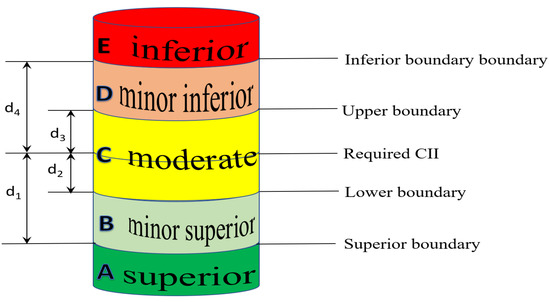
\includegraphics[width=0.5\textwidth]{images/cii_ratings.jpeg}
    \caption{Schematic diagram of the CII ratings and boundaries. \autocite{tsai2023effects}}
    \label{ciiRating}
\end{figure}


The article \cite{rodriguez2020indicators}, discusses the increasing popularity of Energy and Car- bon Intensity indicators among policy makers, which are calculated as units of energy or mass of emissions per unit of Gross Domestic Product (GDP).
These indicators are gaining momen- tum due to support from think tanks, public organizations, consulting groups, and academics focused on energy and climate change policy development.
The ways in which intensity in- dicators are framed and perceived in public debates generated by these intermediaries are important as they can influence policy making and the development of better sets of indicators to assess how well countries are addressing climate change and resource efficiency policies.
Intensity indicators are appealing for emerging economies as they are not incompatible with high rates of economic growth and do not imply the imposition of absolute emission/energy caps.


\subsection{Energy Efficiency Operational Indicator (EEOI)}

The Energy Efficiency Operational Indicator (EEOI) is a tool used to measure the CO2 gas emissions per unit of transport work, indicating the operational efficiency of a ship.
The EEOI is calculated annually and is subject to changes after each voyage due to various external factors, such as navigation conditions, sea area, weather, temperature, and cargo weight.

The EEOI provides an accurate measure for each voyage, and its unit depends on the type of cargo or transport work, such as tons CO2/(tons/nautical miles), tons CO2/(TEU/nautical miles), or tons CO2/(person/nautical miles).
The formula for calculating the EEOI is represented by formula (\ref{eq:eeoi}), where a lower value indicates a more energy-efficient ship \autocite{prill2020new}.

\begin{equation}
    \text{EEOI} = \frac{\text{Carbon Emission}}{\text{Performed Transport Work}}
    \label{eq:eeoi}
\end{equation}

For the calculation of EEOI for a specific voyage, formula (\ref{eq:eeoi_voyage}) is used.

\begin{equation}
    \text{EEOI} = \frac{\sum_{j} F_{Cj} \cdot C_{Fj}}{m_{\text{cargo}} \cdot D_j}
    \label{eq:eeoi_voyage}
\end{equation}

However, when dealing with a large number of ships, formula (\ref{eq:eeoi_voyage}) is expressed as equation (\ref{eq:eeoi_average}), taking into account parameters such as fuel type, voyage number, fuel consumption, fuel-to-CO2 conversion factor, cargo weight, and distance traveled \autocite{tran2017research}.

\begin{equation}
    \text{Average}_{\text{EEOI}} = \frac{\sum_{i}\sum_{j}(F_{C_{i}} \cdot C_{F_{j}})}{\sum_{i}(m_{\text{cargo},i} \cdot D_{i})}
    \label{eq:eeoi_average}
\end{equation}

where:
\begin{align*}
     & j: \text{Fuel type used}                                            \\
     & i: \text{Navigation voyage number}                                  \\
     & FC_{ij}: \text{Mass of consumed fuel } j \text{ at voyage } i       \\
     & CF_{j}: \text{Fuel mass to CO2 mass conversion factor with fuel } j \\
     & m_{cargo}: \text{Weight of cargo carried (tons) on ship}            \\
     & D_{i}: \text{Distance of voyage } i \text{ (nautical miles)}
\end{align*}

The fuel-to-CO2 conversion factor (CF) is a non-dimensional factor that converts fuel consumption, measured in grams, to CO2 gas emissions, also measured in grams, based on the carbon content.
The below table

\ref{tab:fuel_composition} is showed the certain value of CF follows the type of fuel.

\begin{table}[h]
    \centering
    \resizebox{\textwidth}{!}{%
        \begin{tabular}{|c|c|c|c|c|}
            \hline
            \textbf{No.} & \textbf{Type of fuel}         & \textbf{Reference}              & \textbf{Carbon content} & \textbf{CF (t-CO2/t-Fuel)} \\
            \hline
            1            & Diesel/gas oil                & ISO 8217 Grades DMX through DMC & 0.875                   & 3.206000                   \\
            \hline
            2            & Light fuel oil (LFO)          & ISO 8217 Grades RMA through RMD & 0.86                    & 3.151040                   \\
            \hline
            3            & Heavy fuel oil (HFO)          & ISO 8217 Grades RME through RMK & 0.85                    & 3.114400                   \\
            \hline
            4            & Liquefied petroleum gas (LPG) & Propane, butane                 & 0.819, 0.827            & 3.000000, 3.030000         \\
            \hline
            5            & Liquefied natural gas (LNG)   &                                 & 0.75                    & 2.750000                   \\
            \hline
        \end{tabular}
    }
    \caption{The value of CF (t-CO2/t-Fuel) \autocite{tran2017research}.}
    \label{tab:fuel_composition}
\end{table}

\subsection{Energy Efficiency Design Index  (EEDI)}


Energy Efficiency Design Index (EEDI) is a legislation proposed by the International Maritime Organization (IMO) to estimate the energy efficiency of ships and calculate their CO2 emissions per unit of transport work done during the ship design phase.
EEDI is based on a complex formula that takes into account the ship's emissions, capacity, and speed, and the lower the ship's EEDI index, the less CO2 emissions it produces.

EEDI is a non-prescriptive mechanism that allows the shipping industry to use the latest technologies for designing commercial vessels as long as they meet the required energy efficiency levels and parameters.
It lays down a minimum energy efficiency level, per capacity mile, for different ship types and sizes, including tankers, bulk carriers, gas carriers, general cargo ships, container ships, refrigerated cargo carriers, and combination carriers.

The EEDI formula has two components: attained EEDI and required EEDI.
The attained EEDI is calculated using a complex formulation based on the vessel's emissions, capacity, and speed,
while the required EEDI is the minimum level of energy efficiency that a ship must meet as per its ship type and size.
The attained EEDI is verified based on the ship's design and construction, and the required EEDI is the target that the ship must achieve during its operation \autocite{ren2019influence}.

\newpage


EEDI calculation module as part of Marpol Annex VI, following the directive MEPC.1/Circ.681 at the MEPC meeting conducted by the IMO in 2011.
This regulation came into effect on January 1, 2013. The EEDI formula (Equation 1) specified by IMO (2011) is represented by the equation (\ref{eq:attained_eedi}) \autocite{tokucslu2020analyzing}.



\begin{equation}
    EEDI = \frac{{P \cdot \text{SFC} \cdot \text{Cf}}}{{DWT \cdot \text{Vref}}}
    \label{eq:attained_eedi}
\end{equation}


where:
\begin{align*}
    P              & : \text{70\% of the power of the engine (main and auxiliary) in kW}             \\
    \text{SFC}     & : \text{Amount of fuel burned by the engines in kW (specific fuel consumption)} \\
    Cf             & : \text{Emission rate of fuel used by the ship (presented in Table 1)}          \\
    DWT            & : \text{Ship's capacity (in tons)}                                              \\
    V_{\text{ref}} & : \text{Speed of the ship (in knots)}
\end{align*}


\subsection{Energy Efficiency eXisting ship Index  (EEXI)}

The Energy Efficiency Existing Ship Index (EEXI) is a regulation introduced by the International Maritime Organization (IMO) aimed at improving the energy efficiency of existing ships.
It is part of the broader effort to reduce greenhouse gas emissions from the shipping industry and combat climate change.
The EEXI is designed to complement the Energy Efficiency Design Index (EEDI), which focuses on new ship designs \autocite{czermanski2022implementation}.

The EEXI is part of a comprehensive framework that includes short-term, mid-term, and long-term measures.
The short-term measures focus on technical and operational improvements, such as retrofitting ships with energy-efficient technologies.
The mid-term measures involve market-based mechanisms to incentivize emission reductions, while the long-term measures explore alternative fuels and propulsion systems \autocite{CHUAH2023115348}.

The calculation of the Energy Efficiency Existing Ship Index (EEXI) can be optimized by considering the ship's maximum continuous rating (MCR) at 100\% capacity.
This approach ensures that improvements in technical efficiency closely align with the ship's actual operational fuel use.
By accounting for the engine power limits (EPLs) within the engine margin, which have minimal impact on ship operations, a more accurate assessment of energy efficiency can be achieved.
Currently, the proposed calculation methods for the EEXI involve using either 75\% of the limited MCR (MCRlim), similar to the Energy Efficiency Design Index (EEDI), or a higher value of 87\% MCRlim, which only considers the engine margin.
However, utilizing ship characteristics data from IHS Markit and applying the appropriate calculation method, the attained EEXI score can still be estimated, providing valuable insights into a ship's energy performance.

\begin{equation}
    \text{Attained EEXI} = 3.1144 \times \frac{MESFOC \times \sum_{i=1}^{nME} P_{ME,i} + AESFOC \times P_{AE}}{\text{Capacity} \times \text{Vref}}
    \label{eq:attained_eexi}
\end{equation}

The estimation of the attained EEXI score using ship characteristics data from IHS Markit, as outlined in Equation (\ref{eq:attained_eexi}), contributes to a more comprehensive understanding of a ship's energy efficiency.
This information supports decision-making processes related to optimizing operational fuel consumption, implementing retrofit measures, and promoting environmental sustainability in the maritime industry.
By calculating the EEXI at 100\% MCR, the assessment takes into account the EPLs within the engine margin, which are not expected to significantly affect ship operations.
This approach ensures that technical efficiency improvements are properly aligned with the ship's actual operational fuel use, enabling informed decision-making for enhancing operational fuel consumption and reducing environmental impact.
Through the utilization of ship characteristics data and the appropriate calculation method, the attained EEXI score serves as a valuable tool for assessing energy efficiency and driving advancements in the maritime sector.






\section{Problem Statement}

Carbon emissions from maritime shipping have been identified as a major contributor to global greenhouse gas emissions, with the International Maritime Organization estimating that shipping is responsible for around 3\% of global CO2 emissions \autocite{king_anthony_2022}.
To address this issue, the shipping industry has set targets to reduce its carbon footprint, and governments and international organizations have introduced policies and regulations to encourage emissions reduction.

However, measuring and monitoring carbon emissions from maritime shipping can be challenging due to the complexity of the industry and the lack of reliable data.
The Energy Efficiency Existing Ship Index (EEXI) and the Carbon Intensity Indicator (CII) have been proposed as two metrics to assess the carbon efficiency of ships and enable comparison between different vessels and fleets \autocite{ZHANG2019118223,CHUAH2023115348}.
However, there is a need to better understand the relationship between EEXI and carbon emissions, as well as to identify the factors that influence EEXI.

Therefore, the aim of this thesis is to conduct a big data analysis of carbon emissions in maritime shipping, using EEXI as the main metric. Specifically, the study will:

\begin{itemize}
    \item Calculate EEXI for a sample of vessels using real-world data on fuel consumption and other operational parameters.
    \item Analyze the relationship between EEOI, CII, and carbon emissions, using statistical methods and machine learning algorithms.
    \item Identify the factors that influence EEXI and CII, such as vessel age, size, speed, and route, and examine their impact on carbon emissions.
    \item Evaluate the usefulness of EEXI and CII as metrics for monitoring and reducing carbon emissions in maritime shipping, and recommend potential improvements to these metrics.
\end{itemize}


Overall, the findings of this thesis will contribute to a better understanding of the carbon efficiency of maritime shipping and inform the development of policies and strategies for emissions reduction in this sector.
\section{Research Question}

This theis will focus on answering following research questions:

\begin{enumerate}
    \item What is the relationship between vessel age and carbon emissions in maritime shipping?
    \item How do shipping routes affect carbon emissions in maritime shipping?
    \item What role do fuel types and engine technologies play in carbon emissions in maritime shipping?
    \item How can EEOI and CII be used to monitor and reduce carbon emissions in maritime shipping?
\end{enumerate}
\section{Report Outline}

\begin{figure}[ht]
    \centering
    \includegraphics[width=1\textwidth]{images/thesis_outline.png}
    \caption{Outline of the thesis}
    \label{fig:outline}
\end{figure}

\noindent Chapter 2: Litrature Review: This chapter covers the background information and literature review of the thesis.
this section covers comprehensive review of existing papers and research related to carbon emissions in maritime shipping.
The aim is to provide a comprehensive overview of the current state of research in this field and identify any gaps or opportunities for further exploration.


\noindent Chapter 3: Data Collection and Understanding:
In this chapter, the focus will be on gathering and understanding the data required to perform analysis to understand emissions in martime shipping.
Various data sources will be explored, including industry databases, research publications, and government reports.
The aim is to acquire a comprehensive dataset that covers different aspects of carbon emissions in the maritime sector.
Additionally, this chapter will delve into the intricacies of the collected data, understanding its structure, variables, and potential limitations.

\noindent Chapter 4: Data Cleaning and Preprocessing:
Before conducting any data analysis, it is crucial to ensure the quality and integrity of the dataset.
This chapter will discuss the steps involved in cleaning and preprocessing the data.
This process may involve handling missing values, dealing with outliers, standardizing formats, and resolving inconsistencies.
By performing these necessary data cleaning procedures, the dataset will be prepared for further analysis, ensuring reliable and accurate results.

\noindent Chapter 5: Data Analysis Techniques:
In this chapter, various data analysis techniques specific to big data will be explored and applied to the cleaned dataset.
These techniques may include statistical analysis, machine learning algorithms, and data visualization methods.
The goal is to extract meaningful insights and patterns from the data to gain a comprehensive understanding of carbon emissions in maritime shipping.
Additionally, this chapter will discuss the tools and technologies utilized for data analysis and highlight any specific challenges encountered during the process.

\noindent Chapter 6: Evaluation of Results:
After performing the data analysis, this chapter will focus on evaluating and interpreting the obtained results.
The findings will be compared against existing literature, industry benchmarks, and regulatory standards to assess the significance and implications of the analysis.
The strengths and limitations of the analysis approach will be discussed, and recommendations for future research or practical applications will be provided.
This chapter aims to provide a comprehensive evaluation of the insights gained from the data analysis and their potential impact on the maritime shipping industry.

\noindent Conclusion:
The conclusion chapter will summarize the key findings and contributions of the thesis.
It will highlight the significance of the conducted big data analysis on emissions in maritime shipping and its implications for sustainability and environmental initiatives.
The conclusion will also discuss any potential limitations or challenges encountered during the research and suggest avenues for further exploration in this field.